\documentclass[t]{beamer}
\usepackage[
    orientation=landscape,
    size=custom,
    width=25.4,
    height=19.05,
    scale=0.63 % erzeugt 16pt Schriftgröße
]{beamerposter}

\newcommand{\PraesentationSchriftgroesseSehrGross}{\fontsize{30}{45}}
\newcommand{\PraesentationSchriftgroesseGross}{\fontsize{22}{33}}
\newcommand{\PraesentationSchriftgroesseNormal}{\fontsize{16}{29}}
\newcommand{\PraesentationSchriftgroesseKlein}{\fontsize{12}{18}}
\newcommand{\PraesentationSchriftgroesseDreizeiler}{\fontsize{7}{10}}
\newcommand{\PraesentationSchriftgroesseAufzaehlungszeichen}{\fontsize{10}{8}}

\newcommand{\PraesentationAbstandAbsatz}{22.1pt}
\newcommand{\PraesentationPositionKorrekturOben}{-1.8cm}
\newcommand{\PraesentationBeispieleSchriftgroessen}{30 | 22 | 16 | 12}

\usepackage[ascii]{inputenc}
%\usepackage[T1]{fontenc} % Zeichensatzkodierung

\usepackage{calc} % Berechnungen

\usepackage{mathtools}

\usepackage[english]{babel}
\usepackage{graphicx}
\usepackage[caption=false]{subfig}
\usepackage[export]{adjustbox}
\usepackage[absolute, overlay]{textpos} % Positionierung

% Silbentrennung:
\usepackage{hyphenat}

% Euro-Symbol:
\usepackage[gen]{eurosym}
\DeclareUnicodeCharacter{20AC}{\euro{}}

% Schriftart Helvetica:
\usepackage[scaled]{helvet}
\renewcommand{\familydefault}{\sfdefault}

\usepackage{mathptmx} % skalierbare Formelschriften

\usepackage{tabularx}

\usepackage{multicol} % mehrspaltiger Text

\usepackage{tikz}
\usetikzlibrary{arrows, shapes, shapes.multipart, trees, positioning, backgrounds, fit, matrix, calc, decorations.pathreplacing, decorations.pathmorphing}

\usepackage[
    bibencoding=utf8,
    style=verbose,
    bibstyle=authoryear,
    maxnames=3,
    giveninits=true,
    uniquename=init,
    ]{biblatex}

\DeclareNameAlias{sortname}{family-given}
\addbibresource{references.bib}

\usepackage{braket}

%% Diagramme:
%\usepackage{pgfplots}
%\pgfplotsset{compat=default}

% Erweiterbare Fusszeile:
\newcommand{\PraesentationFusszeileZusatz}{}

\newcommand{\N}{{\mathbb{N}}}
\newcommand{\R}{{\mathbb{R}}}
\newcommand{\C}{{\mathbb{C}}}

\newcommand{\ud}{\mathrm{d}}

\DeclarePairedDelimiter\abs{\lvert}{\rvert}
\DeclarePairedDelimiter\norm{\lVert}{\rVert}

\DeclareMathOperator{\e}{e}
\DeclareMathOperator{\tr}{tr}
\DeclareMathOperator{\argmin}{argmin}

\newcommand{\highlight}[1]{\mathbf{\color{TUMOrange}#1}}

\graphicspath{{figures/}}


% Für die Person anpassen:
\newcommand{\PersonTitel}{Prof.~Dr.}
\newcommand{\PersonVorname}{Christian B.}
\newcommand{\PersonNachname}{Mendl}

% Fakultät:
\newcommand{\FakultaetName}{CIT, Department of Computer Science}
\newcommand{\LehrstuhlName}{Chair of Scientific Computing -- Quantum Computing}

\newcommand{\Datum}{\today}

\renewcommand{\PraesentationFusszeileZusatz}{| Quantum Simulation and Tensor Network Methods}

\title{Quantum Simulation and Tensor Network Methods}
\author{\PersonTitel{} \PersonVorname{} \PersonNachname}
\institute[]{\UniversitaetName \\ \FakultaetName \\ \LehrstuhlName}
\date[\Datum]{April 22, 2023 \\ $ $ \\ \textbf{45.~Edgar-L\"uscher-Seminar am Gymnasium Zwiesel}\\ \textbf{Quantenphysik in der Anwendung}\\[1cm]

\includegraphics[width=4cm]{qr_github_repo.png}}


% Allgemein:
\newcommand{\AllgemeinGestalter}{ediundsepp Gestaltungsgesellschaft}
\newcommand{\AllgemeinErsteller}{eWorks GmbH}

% Universität:
\newcommand{\UniversitaetName}{Technische Universit\"at M\"unchen}
\newcommand{\UniversitaetAbkuerzung}{TUM}
\newcommand{\UniversitaetWebseite}{www.tum.de}
\newcommand{\UniversitaetLogoBreite}{19mm}
\newcommand{\UniversitaetLogoHoehe}{1cm}

\newcommand{\PraesentationSeitenrand}{8.9mm}
\newcommand\crule[3][black]{\textcolor{#1}{\rule{#2}{#3}}}

\newlength\smallerbaselineskip
\setlength{\smallerbaselineskip}{0.8\baselineskip}

    % Blautöne:
\definecolor{TUMBlau}{RGB}{0,101,189} % Pantone 300
\definecolor{TUMBlauDunkel}{RGB}{0,82,147} % Pantone 301
\definecolor{TUMBlauHell}{RGB}{152,198,234} % Pantone 283
\definecolor{TUMBlauMittel}{RGB}{100,160,200} % Pantone 542

    % Hervorhebung:
\definecolor{TUMElfenbein}{RGB}{218,215,203} % Pantone 7527 -Elfenbein
\definecolor{TUMGruen}{RGB}{162,173,0} % Pantone 383 - Grün
\definecolor{TUMOrange}{RGB}{227,114,34} % Pantone 158 - Orange
\definecolor{TUMGrau}{gray}{0.6} % Grau 60%

\definecolor{forestgreen}{rgb}{.132,.545,.132}


\setbeamercolor*{alerted text}{fg=TUMOrange}

\newcommand{\PraesentationSetzeTextfarbe}{%
    \color{PraesentationTextfarbe}%
    \setbeamercolor*{frametitle}{fg=PraesentationTextfarbe}%
    \setbeamercolor*{normal text}{fg=PraesentationTextfarbe}%
    \setbeamercolor{itemize/enumerate body}{fg=PraesentationTextfarbe}%
    \setbeamercolor*{itemize item}{fg=PraesentationTextfarbe}%
    \setbeamercolor*{itemize subitem}{fg=PraesentationTextfarbe}%
}

\newcommand{\PraesentationFarbschemaStandard}{%
    \setbeamercolor*{background canvas}{}%
    \definecolor{PraesentationTextfarbe}{rgb}{0,0,0}%
    \PraesentationSetzeTextfarbe%
}

\newcommand{\PraesentationFarbschemaWeissBlau}{%
    \setbeamercolor*{background canvas}{bg=TUMBlauDunkel}%
    \definecolor{PraesentationTextfarbe}{rgb}{1,1,1}%
    \PraesentationSetzeTextfarbe%
}

\newcommand{\PraesentationFarbschemaWeissSchwarz}{%
    \setbeamercolor*{background canvas}{bg=black}%
    \definecolor{PraesentationTextfarbe}{rgb}{1,1,1}%
    \PraesentationSetzeTextfarbe%
}

\newcommand{\PraesentationTitelseiteInhalt}{%
    \begin{textblock*}{\paperwidth}[0,0](0cm,-\PraesentationSeitenrand - 6.5mm + \PraesentationPositionKorrekturOben)%
        \color{PraesentationTextfarbe}%
        \frametitle{\inserttitle}
        \vspace*{49.4mm}%
        \usebeamerfont{author}\selectfont\insertauthor\\%
        \insertinstitute\\%
        \insertdate%
    \end{textblock*}%
}

\newcommand{\PraesentationSeitenkopfInhalt}[1]{%
    %\vspace*{31.7mm}%
    \begin{textblock*}{1.68cm}[1,0](\paperwidth - \PraesentationSeitenrand - \PraesentationSeitenrand, 0cm)%
        \includegraphics[width=1.68cm]{#1}%
    \end{textblock*}%
    \begin{textblock*}{3cm}[1,0](\paperwidth - \PraesentationSeitenrand, -\PraesentationSeitenrand)%
        \hbox{%
            \color{PraesentationTextfarbe}%
            \hbox{\insertframenavigationsymbol}%
            \hbox{\insertsubsectionnavigationsymbol}%
            \hbox{\insertsectionnavigationsymbol}%
        }%
    \end{textblock*}%
}

\newcommand{\PraesentationBildUhrenturm}{%
    \begin{textblock*}{10.82cm}[1,1](\paperwidth - \PraesentationSeitenrand - \PraesentationSeitenrand, \paperheight - 9mm)%
        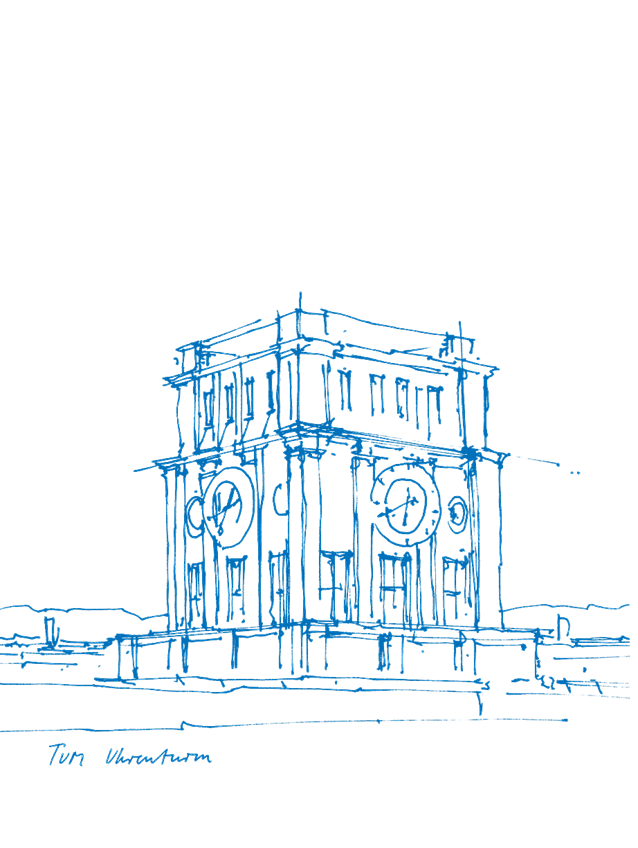
\includegraphics{TUM_Uhrenturm.png}%
    \end{textblock*}%
}

\newcommand{\PraesentationStartseiteUhrenturm}{%
    \setbeamertemplate{title page}{%
        \PraesentationSeitenkopfInhalt{Universitaet_Logo_RGB.pdf}%
        \PraesentationBildUhrenturm%
        \PraesentationTitelseiteInhalt%
    }%
}

\newcommand{\PraesentationStartseiteFlaggen}{%
    \setbeamertemplate{title page}{%
        \begin{textblock*}{\paperwidth}[0,1](-\PraesentationSeitenrand,\paperheight-\PraesentationSeitenrand)%
            
\includegraphics[min width=\paperwidth,max width=\paperheight,min totalsize={\paperwidth}{\paperheight},keepaspectratio,center]{Universitaet_Flaggen.jpg}%
        \end{textblock*}%
        \PraesentationSeitenkopfInhalt{Universitaet_Logo_weiss.pdf}%
        \PraesentationTitelseiteInhalt%
    }%
}

\newcommand{\PraesentationStartseiteLeer}{%
    \setbeamertemplate{title page}{%
        \PraesentationSeitenkopfInhalt{Universitaet_Logo_weiss.pdf}%
        \PraesentationTitelseiteInhalt%
    }%
}


\newcommand{\PraesentationMasterStandard}{%
    \PraesentationFarbschemaStandard%
    \PraesentationStartseiteUhrenturm%
    \setbeamertemplate{headline}{%
        \PraesentationSeitenkopfInhalt{Universitaet_Logo_RGB.pdf}%
    }%
}

\newcommand{\PraesentationMasterWeissBlau}{%
    \PraesentationFarbschemaWeissBlau%
    \PraesentationStartseiteLeer%
    \setbeamertemplate{headline}{%
        \PraesentationSeitenkopfInhalt{Universitaet_Logo_weiss.pdf}%
    }%
}


\newcommand{\PraesentationMasterWeissSchwarz}{%
    \PraesentationFarbschemaWeissSchwarz%
    \setbeamertemplate{title page}{%
        \PraesentationTitelseiteInhalt%
        \PraesentationSeitenkopfInhalt{Universitaet_Logo_weiss.pdf}%
    }
    \setbeamertemplate{headline}{%
        \PraesentationSeitenkopfInhalt{Universitaet_Logo_weiss.pdf}%
    }
}

\newcommand{\PraesentationTitelseite}{\frame[plain]{\titlepage}}
\newcommand{\PraesentationUeberschriftZweizeilig}[2]{\frametitle{#1\\[8mm]#2}}

\setbeamersize{
    text margin left=\PraesentationSeitenrand,
    text margin right=\PraesentationSeitenrand
}

\setbeamertemplate{frametitle}{%
    {\rule{0pt}{42mm + \PraesentationPositionKorrekturOben}\PraesentationSchriftgroesseSehrGross\selectfont\insertframetitle\newline\vspace*{-6.7mm}}%
}

% Aufzählungen:
\newcommand{\PraesentationAufzaehlungEbeneEinsSymbol}{\raise2pt\hbox{\donotcoloroutermaths\usebeamercolor{itemize subitem}\PraesentationSchriftgroesseAufzaehlungszeichen$\bullet$}}
\newcommand{\PraesentationAufzaehlungEbeneZweiSymbol}{\raise1.25pt\hbox{\donotcoloroutermaths\usebeamercolor{itemize subitem}$-$}}
\setbeamertemplate{itemize items}[circle]
\setbeamertemplate{itemize subitem}[triangle]
\setbeamercolor{itemize subitem}{fg=black}
\setbeamerfont{itemize/enumerate subbody}{size=\normalsize}
\setbeamertemplate{itemize item}{\PraesentationAufzaehlungEbeneEinsSymbol}
\setbeamertemplate{itemize subitem}{\PraesentationAufzaehlungEbeneZweiSymbol{}}
%\addtolength{\leftmarginii}{16mm-2pt}%

\newenvironment{PraesentationAufzaehlung}
{%
    \vspace{-\baselineskip}%
    \begin{itemize}%
        \setlength{\itemsep}{0pt}%
        \setlength{\parskip}{0pt}%
        \setlength{\parsep}{0pt}%
        \addtolength{\itemindent}{-1ex}%
}{%
    \end{itemize}%
}


% PDF-Einstellungen:
\hypersetup{
    pdfstartview={Fit},
    pdfproducer={\AllgemeinErsteller},
    pdfcreator={\AllgemeinGestalter}
}

\textblockorigin{\PraesentationSeitenrand}{\PraesentationSeitenrand} % Ursprung für Positionierung

\setbeamerfont{footnote}{size=\PraesentationSchriftgroesseKlein}

\setbeamertemplate{footline}{
    \hbox{%
        \usebeamerfont{footnote}%
        \begin{beamercolorbox}[wd=.9\paperwidth]{}%
            \hspace*{\PraesentationSeitenrand}%
            \PersonTitel{} \PersonVorname~\PersonNachname~(\UniversitaetAbkuerzung) \PraesentationFusszeileZusatz{}%
        \end{beamercolorbox}%
        \begin{beamercolorbox}[wd=.1\paperwidth]{}%
            \insertframenumber{}%
            \raggedleft
            \hspace*{\PraesentationSeitenrand}%
        \end{beamercolorbox}%
        \vspace*{3.25mm}%
    }%
}

\setbeamertemplate{navigation symbols}{}


\begin{document}
\setlength{\baselineskip}{\PraesentationAbstandAbsatz}
\setlength{\parskip}{\baselineskip}


\PraesentationMasterStandard

\PraesentationTitelseite



\begin{frame}
\frametitle{Motivation: Simulate quantum systems}
Strangeness of strongly correlated quantum systems, still unsolved questions:
\begin{tabular}{cccc}
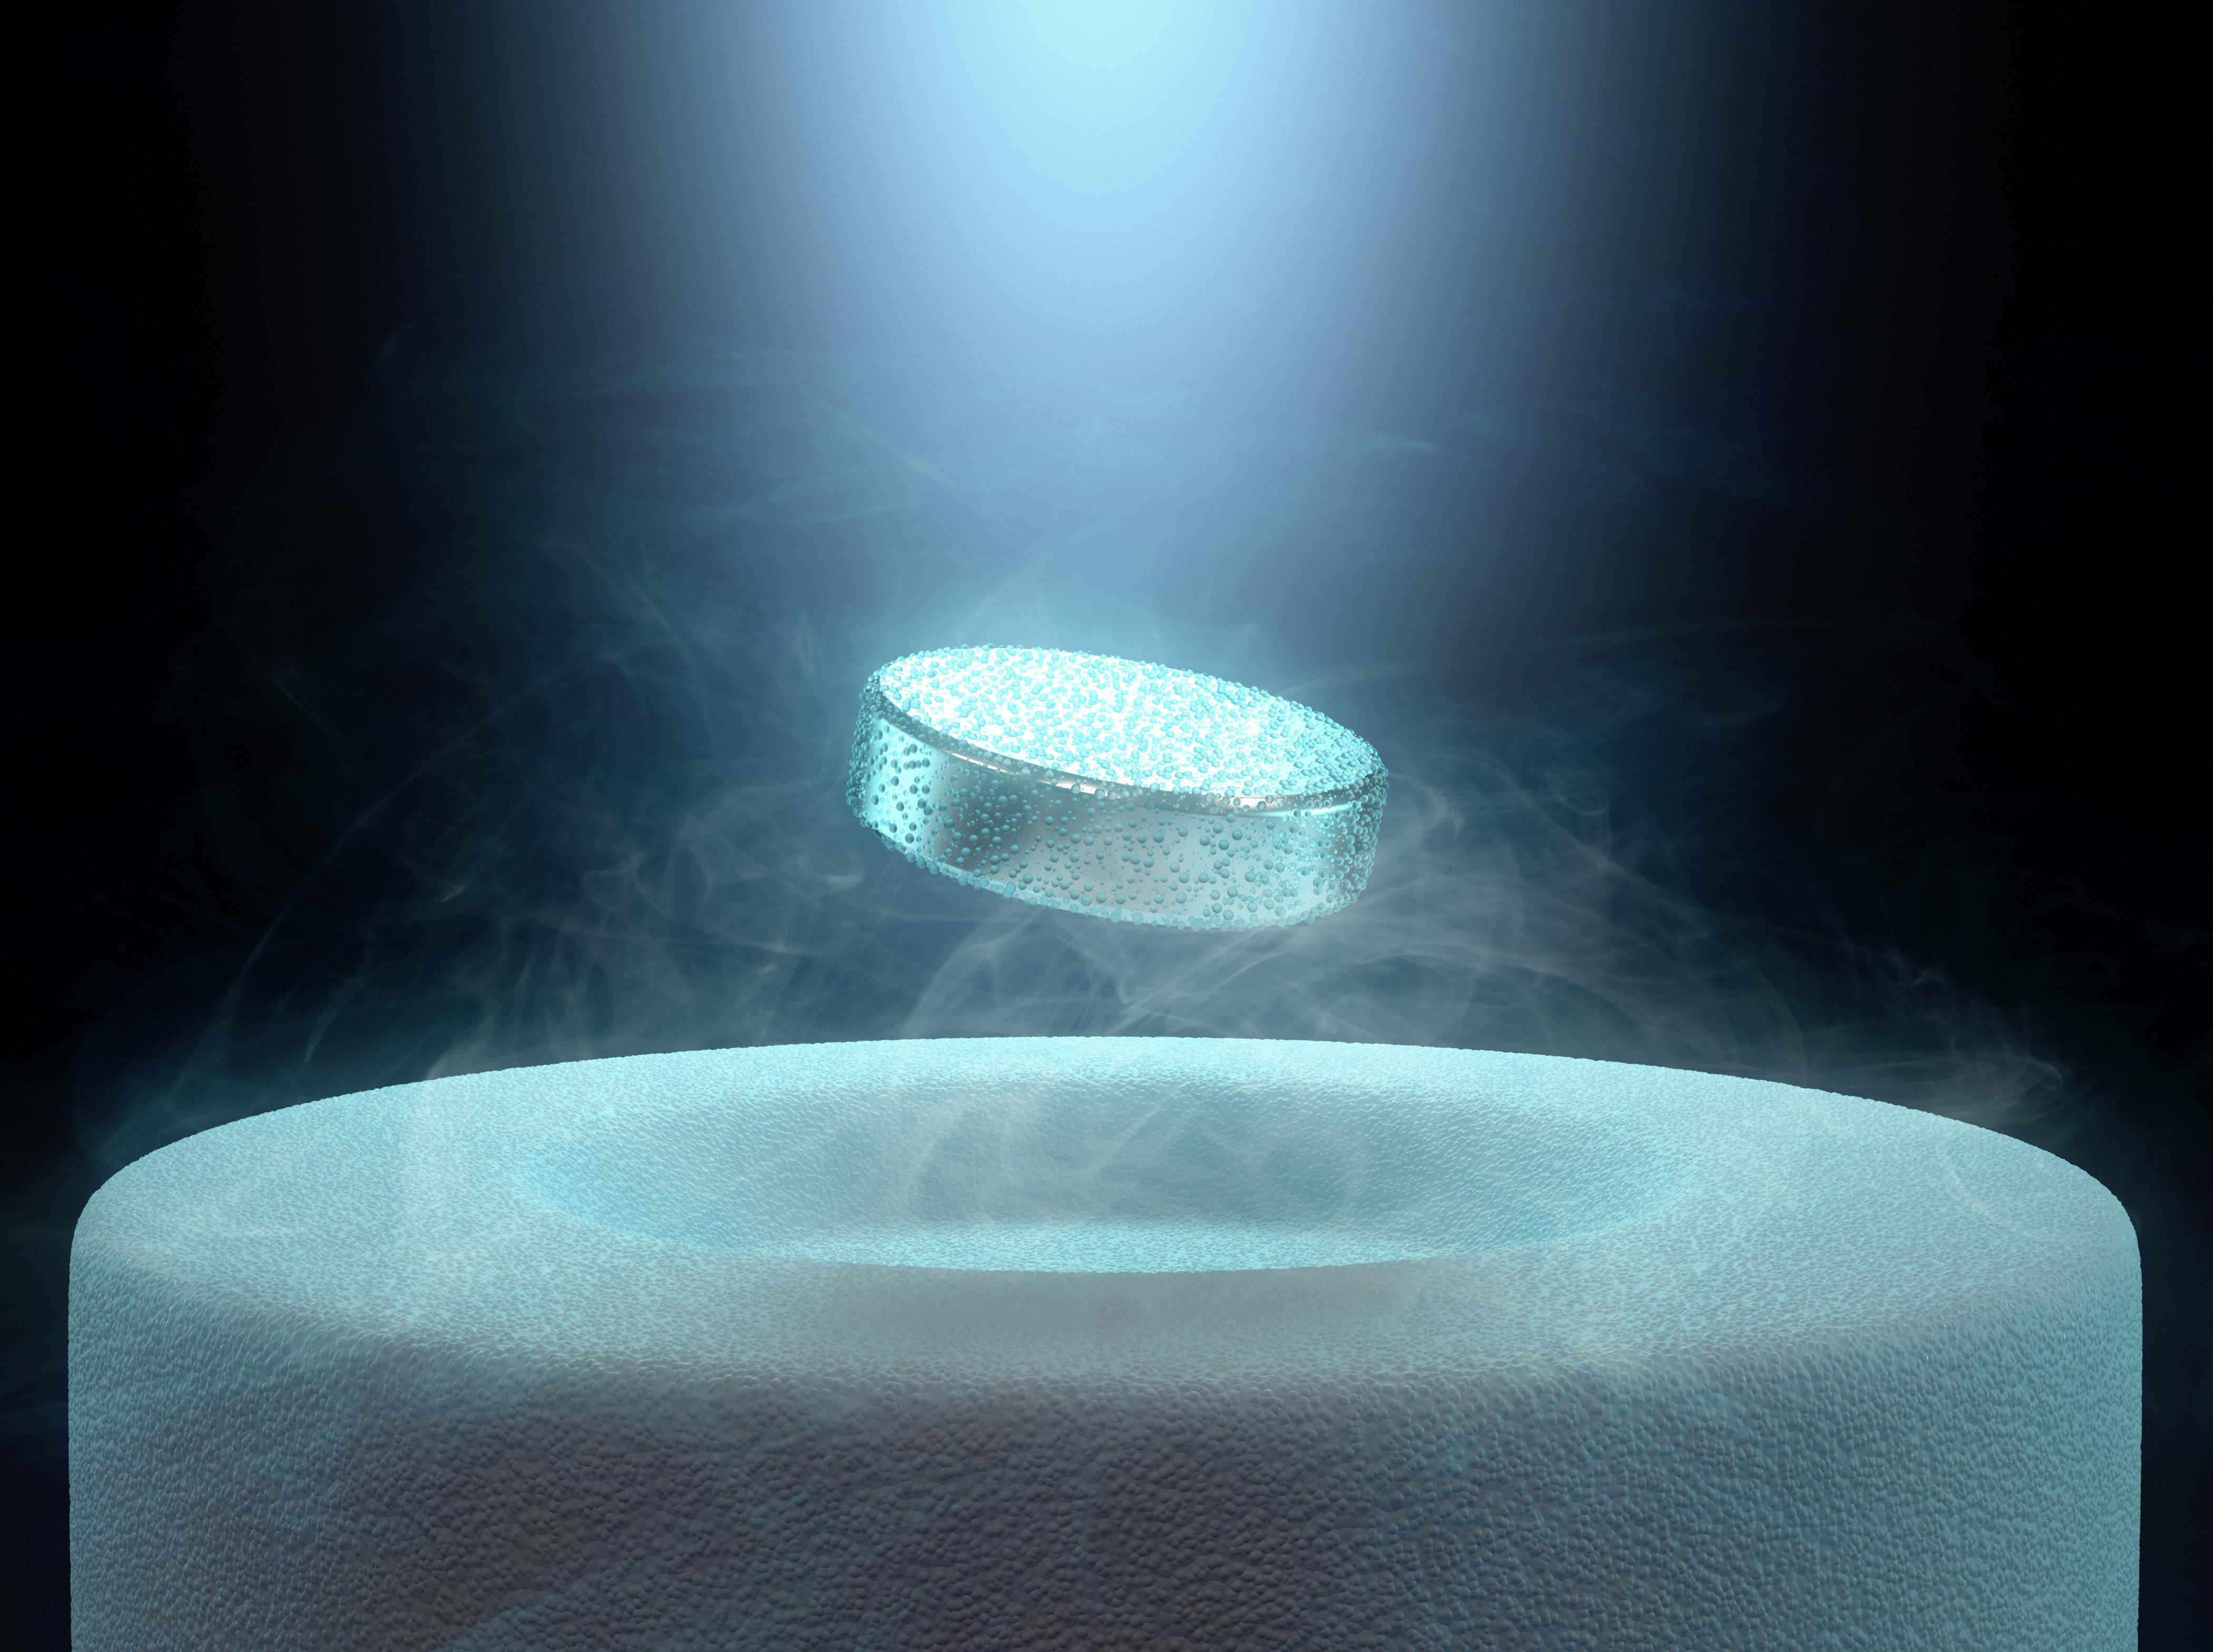
\includegraphics[width=0.3\textwidth]{superconductor.jpg} & 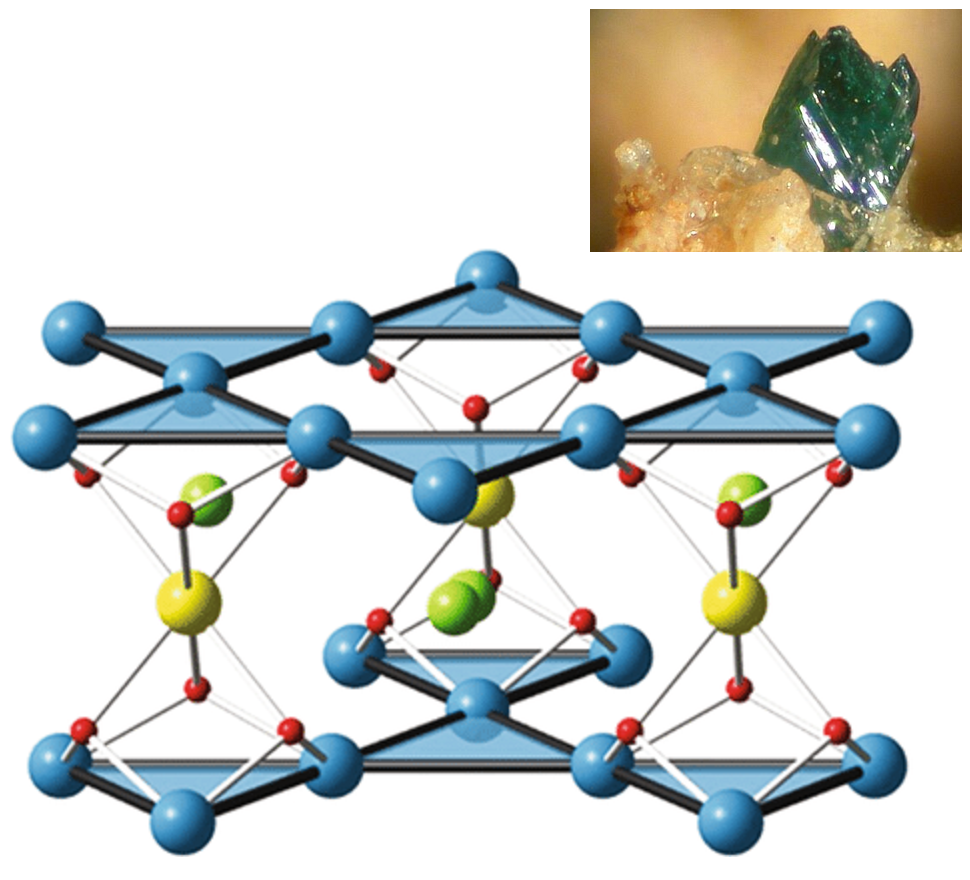
\includegraphics[width=0.3\textwidth]{herbertsmithite_combined.png} & 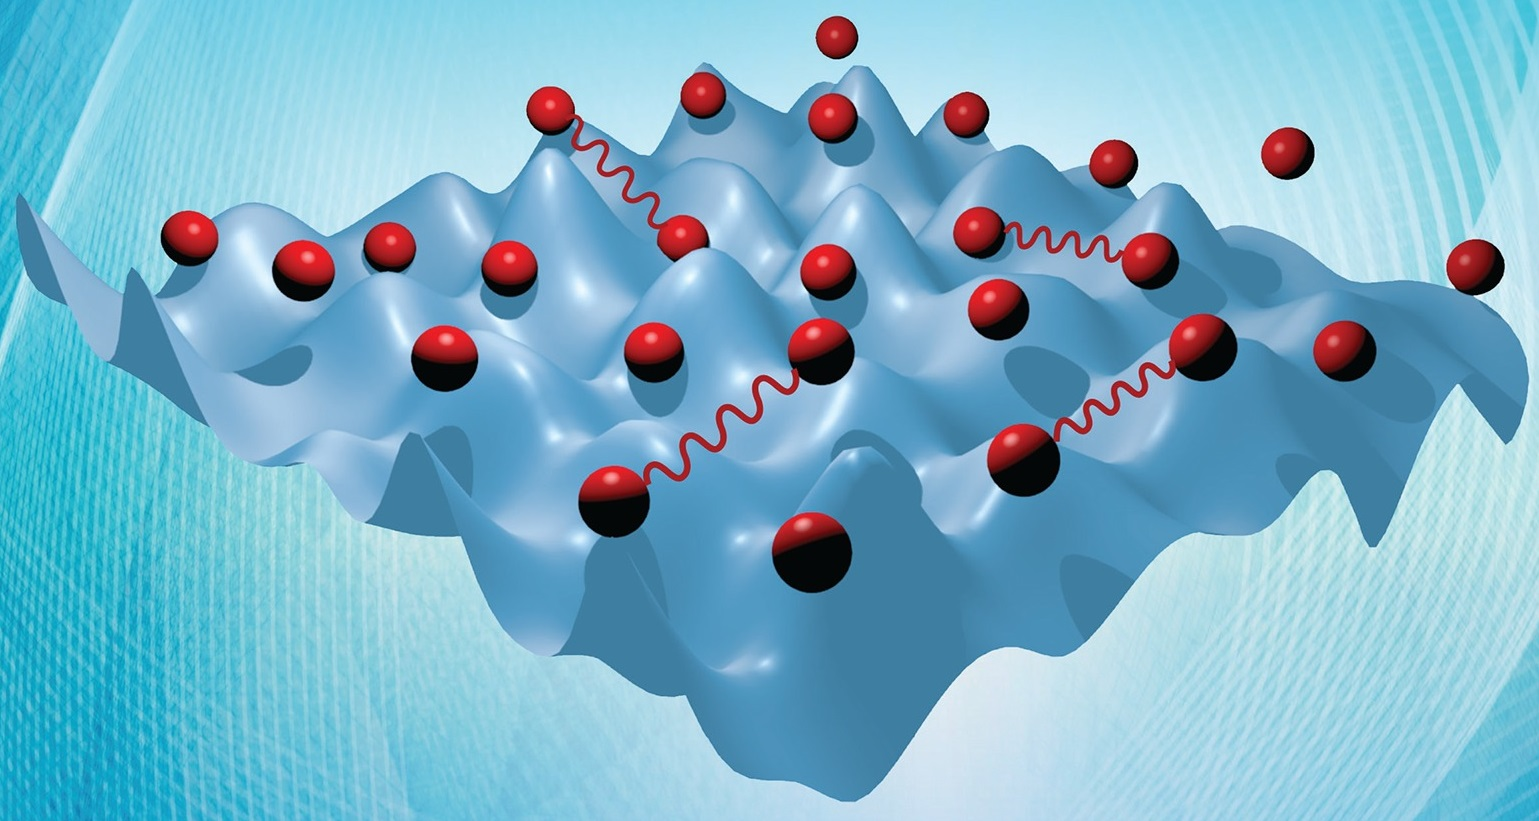
\includegraphics[width=0.3\textwidth]{many_body_localization.jpg} \\
high-$T_c$ superconductors & Novel quantum phases & Many-body localization
\end{tabular}

\begin{minipage}[t]{0.6\textwidth}%
Electronic Schr\"odinger equation:
\[
H\,\psi = E \psi
\]
Quantum Hamiltonian $H$:
\[
H = -\sum_{j = 1}^{{\color{TUMBlau}N}} \frac{\hbar^2}{2 m_{\mathrm{e}}} \nabla_{r_j}^2 + \sum_{j < k}^{{\color{TUMBlau}N}} \frac{\mathrm{e}^2}{4 \pi \epsilon_0 \abs{r_j - r_k}} - \sum_{j = 1}^M \sum_{k = 1}^{{\color{TUMBlau}N}} \frac{Z_j \mathrm{e}^2}{4 \pi \epsilon_0 \abs{R_j - r_k}}
\]
$\{ R_j \}$: positions of atomic nuclei, $\{ r_j \}$: electron positions
\end{minipage}%
\hspace{0.05\textwidth}%
\begin{minipage}[t]{0.3\textwidth}%
\begin{figure}
\centering
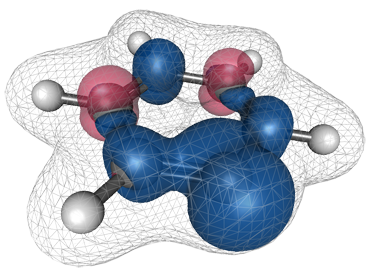
\includegraphics[width=\textwidth]{molecule.png}\\
{\footnotesize Source: \href{http://iqmol.org}{iqmol.org}}
\end{figure}
\end{minipage}
\end{frame}



\PraesentationMasterWeissBlau

\begin{frame}
\vspace{7cm}
\begin{center}
{\LARGE Qubitization and quantum eigenvalue transforms}

\[
U_{\vec{\varphi}} = \e^{i \varphi_0 Z} \prod_{k=1}^d W(a) \e^{i \varphi_k Z}
\]
\end{center}
\end{frame}

\PraesentationMasterStandard



\begin{frame}
\frametitle{Quantum signal processing (QSP)}
Goal: realize a function $f({\color{TUMBlau}a})$ using single-qubit gates \\
Alternating sequence of single-qubit rotation operators:\\
\begin{itemize}
\item ``\alert{signal} rotation operator'', for ${\color{TUMBlau}a} \in [-1, 1]$:
\[
W({\color{TUMBlau}a}) = \begin{pmatrix} {\color{TUMBlau}a} & i \sqrt{1 - {\color{TUMBlau}a}^2} \\ i \sqrt{1 - {\color{TUMBlau}a}^2} & {\color{TUMBlau}a} \end{pmatrix}
\]
\item ``\alert{signal-processing} rotation operator'', with $Z = \left(\begin{smallmatrix} 1 & 0 \\ 0 & -1 \end{smallmatrix}\right)$:
\[
S({\color{forestgreen}\varphi}) = \e^{i {\color{forestgreen}\varphi} Z}, \quad {\color{forestgreen}\varphi} \in \R
\]
\end{itemize}
%
For phases ${\color{forestgreen}\vec{\varphi}} = ({\color{forestgreen}\varphi_0}, \dots, {\color{forestgreen}\varphi_d}) \in \R^{d+1}$, define
\[
U_{\color{forestgreen}\vec{\varphi}} = \e^{i {\color{forestgreen}\varphi_0} Z} W({\color{TUMBlau}a}) \e^{i {\color{forestgreen}\varphi_1} Z} W({\color{TUMBlau}a}) \cdots \e^{i {\color{forestgreen}\varphi_d} Z} = \e^{i {\color{forestgreen}\varphi_0} Z} \prod_{k=1}^d W({\color{TUMBlau}a}) \e^{i {\color{forestgreen}\varphi_k} Z}
\]
%
Examples:
\vspace{3cm}

\footnotesize{%
{\usebeamercolor[fg]{structure}J.~M.~Martyn et al.} ``Grand unification of quantum algorithms''. PRX Quantum, 040203 (2021)\nocite{Martyn2021}\\
{\usebeamercolor[fg]{structure}G.~H.~Low and I.~L.~Chuang}. ``Hamiltonian simulation by qubitization''. Quantum 3, 163 (2019)\nocite{Low2019}}
\end{frame}



\begin{frame}
\frametitle{Quantum signal processing theorem}
\vspace{1cm}
\begin{theorem}[Quantum signal processing] The QSP sequence $U_{\vec{\varphi}}$ produces a matrix that maybe be expressed as polynomial function of ${\color{TUMBlau}a}$:
\[
U_{\color{forestgreen}\vec{\varphi}} = \e^{i {\color{forestgreen}\varphi_0} Z} \prod_{k=1}^d W({\color{TUMBlau}a}) \e^{i {\color{forestgreen}\varphi_k} Z} = \begin{pmatrix} P({\color{TUMBlau}a}) & i Q({\color{TUMBlau}a}) \sqrt{1 - {\color{TUMBlau}a}^2} \\ i Q^*({\color{TUMBlau}a}) \sqrt{1 - {\color{TUMBlau}a}^2} & P^*({\color{TUMBlau}a}) \end{pmatrix}
\]
for ${\color{TUMBlau}a} \in [-1, 1]$, and a ${\color{forestgreen}\vec{\varphi}}$ exists for any polynomials $P$, $Q$ such that:
\begin{enumerate}
\item[(i)] $\deg(P) \le d$, $\deg(Q) \le d-1$
\item[(ii)] $P$ has parity $d \!\!\mod 2$ and $Q$ has parity $(d-1) \!\!\mod 2$
\item[(iii)] $\abs{P({\color{TUMBlau}a})}^2 + (1 - {\color{TUMBlau}a}^2) \abs{Q({\color{TUMBlau}a})}^2$ = 1
\end{enumerate}
\end{theorem}

\footnotesize{%
{\usebeamercolor[fg]{structure}J.~M.~Martyn et al.} ``Grand unification of quantum algorithms''. PRX Quantum, 040203 (2021)\nocite{Martyn2021} \\
\url{https://github.com/ichuang/pyqsp} \\
\url{https://github.com/qsppack/QSPPACK}
}
\end{frame}



\begin{frame}
\frametitle{Qubitization illustrated by amplitude amplification}
Given:\\
\begin{itemize}
\item (black box) unitary operator $U$
\item quantum state $\ket{A_0}$, $\ket{B_0}$ with ${\color{TUMBlau}a} := \braket{A_0 \vert U \vert B_0} \neq 0$ (w.l.o.g.\ ${\color{TUMBlau}a} \in \R$)
\item corresponding phase rotation gates
\[
A_{\color{forestgreen}\varphi} = \e^{i {\color{forestgreen}\varphi} \ket{A_0}\bra{A_0}}, \quad B_{\color{forestgreen}\varphi} = \e^{i {\color{forestgreen}\varphi} \ket{B_0}\bra{B_0}}
\]
\end{itemize}
Goal: construct quantum circuit $C$ from $U$, $U^{\dagger}$, $A_{\color{forestgreen}\varphi}$, $B_{\color{forestgreen}\varphi}$ such that $\abs{\braket{A_0 \vert C \vert B_0}} \to 1$

\begin{flushright}
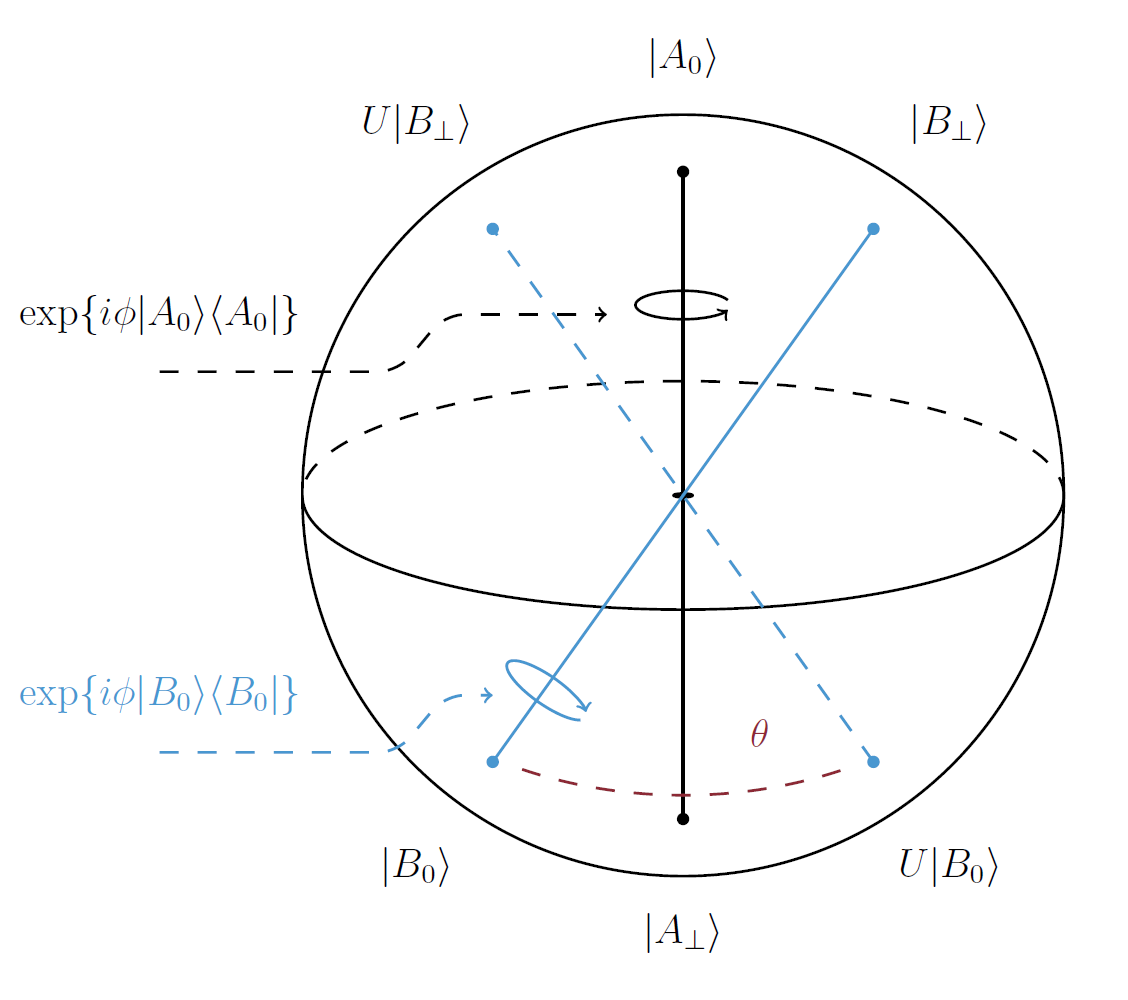
\includegraphics[width=0.4\textwidth]{qubitization_amplitude_amplification.png}
\end{flushright}
\end{frame}



\begin{frame}
\frametitle{Quantum eigenvalue transforms}
So far: QSP with parameter ${\color{TUMBlau}a} \in [-1, 1]$\\
It turns out: can apply QSP to all eigenvalues $\{ {\color{TUMBlau}\lambda_j} \}$ of a Hermitian matrix $H$ simultaneously, with ``${\color{TUMBlau}a} = {\color{TUMBlau}\lambda_j}$''

Strategy: \alert{block-encode} $H$ into a larger unitary matrix $V$:

\vspace{5cm}

\[
V = \sum_j \ \raisebox{-15mm}{\begin{tikzpicture}[scale=1.750000,x=1pt,y=1pt]
\filldraw[color=white] (0.000000, -7.500000) rectangle (47.000000, 52.500000);
% Drawing wires
% Line 2: color=TUMOrange a W
\draw[color=TUMOrange] (0.000000,45.000000) -- (47.000000,45.000000);
% Line 3: b W
\draw[color=black] (0.000000,30.000000) -- (47.000000,30.000000);
% Line 4: c W
\draw[color=black] (0.000000,15.000000) -- (47.000000,15.000000);
% Line 5: d W
\draw[color=black] (0.000000,0.000000) -- (47.000000,0.000000);
% Done with wires; drawing gates
% Line 6: a G $R(\lambda_j)$ width=24 fill=TUMBlauHell
\begin{scope}
\draw[fill=TUMBlauHell] (23.500000, 45.000000) +(-45.000000:16.970563pt and 8.485281pt) -- +(45.000000:16.970563pt and 8.485281pt) -- +(135.000000:16.970563pt and 8.485281pt) -- +(225.000000:16.970563pt and 8.485281pt) -- cycle;
\clip (23.500000, 45.000000) +(-45.000000:16.970563pt and 8.485281pt) -- +(45.000000:16.970563pt and 8.485281pt) -- +(135.000000:16.970563pt and 8.485281pt) -- +(225.000000:16.970563pt and 8.485281pt) -- cycle;
\draw (23.500000, 45.000000) node {$R(\lambda_j)$};
\end{scope}
% Line 7: b c d G $\ket{\psi_j}\bra{\psi_j}$ width=35
\draw (23.500000,30.000000) -- (23.500000,0.000000);
\begin{scope}
\draw[fill=white] (23.500000, 15.000000) +(-45.000000:24.748737pt and 29.698485pt) -- +(45.000000:24.748737pt and 29.698485pt) -- +(135.000000:24.748737pt and 29.698485pt) -- +(225.000000:24.748737pt and 29.698485pt) -- cycle;
\clip (23.500000, 15.000000) +(-45.000000:24.748737pt and 29.698485pt) -- +(45.000000:24.748737pt and 29.698485pt) -- +(135.000000:24.748737pt and 29.698485pt) -- +(225.000000:24.748737pt and 29.698485pt) -- cycle;
\draw (23.500000, 15.000000) node {$\ket{\psi_j}\bra{\psi_j}$};
\end{scope}
% Done with gates; drawing ending labels
% Done with ending labels; drawing cut lines and comments
% Done with comments
\end{tikzpicture}
}
\]
\footnotesize{%
{\usebeamercolor[fg]{structure}J.~M.~Martyn et al.} ``Grand unification of quantum algorithms''. PRX Quantum, 040203 (2021)\nocite{Martyn2021}\\
{\usebeamercolor[fg]{structure}G.~H.~Low and I.~L.~Chuang}. ``Hamiltonian simulation by qubitization''. Quantum 3, 163 (2019)\nocite{Low2019}\\
{\usebeamercolor[fg]{structure}A.~Gily\'{e}n et al.} ``Quantum singular value transformation and beyond: exponential improvements for quantum matrix arithmetics''. STOC 2019\nocite{Gilyen2019}%
}
\end{frame}



\begin{frame}
\frametitle{Quantum eigenvalue transforms (cont.)}
Apply QSP sequence to auxiliary qubit $\leadsto$ transforms all eigenvalues simultaneously!

\[
U_{{\color{forestgreen}\vec{\varphi}}, \text{eig}} = \e^{i {\color{forestgreen}\varphi_0} Z} \prod_{k=1}^d V \e^{i {\color{forestgreen}\varphi_k} Z} = \begin{pmatrix} \mathrm{Poly}({\color{TUMBlau}H}) & \cdot \\ \cdot & \cdot \end{pmatrix}
\]

\[
\raisebox{-13mm}{\begin{tikzpicture}[scale=1.750000,x=1pt,y=1pt]
\filldraw[color=white] (0.000000, -7.500000) rectangle (191.000000, 52.500000);
% Drawing wires
% Line 2: color=TUMOrange a W \ket{0} \bra{0}
\draw[color=TUMOrange] (0.000000,45.000000) -- (191.000000,45.000000);
\draw[color=TUMOrange] (0.000000,45.000000) node[left] {$\ket{0}$};
% Line 3: b W
\draw[color=black] (0.000000,30.000000) -- (191.000000,30.000000);
% Line 4: c W
\draw[color=black] (0.000000,15.000000) -- (191.000000,15.000000);
% Line 5: d W
\draw[color=black] (0.000000,0.000000) -- (191.000000,0.000000);
% Done with wires; drawing gates
% Line 6: a G $\e^{i {\color{forestgreen}\varphi_0}}$ width=18
\begin{scope}
\draw[fill=white] (15.000000, 45.000000) +(-45.000000:12.727922pt and 8.485281pt) -- +(45.000000:12.727922pt and 8.485281pt) -- +(135.000000:12.727922pt and 8.485281pt) -- +(225.000000:12.727922pt and 8.485281pt) -- cycle;
\clip (15.000000, 45.000000) +(-45.000000:12.727922pt and 8.485281pt) -- +(45.000000:12.727922pt and 8.485281pt) -- +(135.000000:12.727922pt and 8.485281pt) -- +(225.000000:12.727922pt and 8.485281pt) -- cycle;
\draw (15.000000, 45.000000) node {$\e^{i {\color{forestgreen}\varphi_0}}$};
\end{scope}
% Line 7: a b c d G $V$ width=25
\draw (48.500000,45.000000) -- (48.500000,0.000000);
\begin{scope}
\draw[fill=white] (48.500000, 22.500000) +(-45.000000:17.677670pt and 40.305087pt) -- +(45.000000:17.677670pt and 40.305087pt) -- +(135.000000:17.677670pt and 40.305087pt) -- +(225.000000:17.677670pt and 40.305087pt) -- cycle;
\clip (48.500000, 22.500000) +(-45.000000:17.677670pt and 40.305087pt) -- +(45.000000:17.677670pt and 40.305087pt) -- +(135.000000:17.677670pt and 40.305087pt) -- +(225.000000:17.677670pt and 40.305087pt) -- cycle;
\draw (48.500000, 22.500000) node {$V$};
\end{scope}
% Line 8: a G $\e^{i {\color{forestgreen}\varphi_1}}$ width=18
\begin{scope}
\draw[fill=white] (82.000000, 45.000000) +(-45.000000:12.727922pt and 8.485281pt) -- +(45.000000:12.727922pt and 8.485281pt) -- +(135.000000:12.727922pt and 8.485281pt) -- +(225.000000:12.727922pt and 8.485281pt) -- cycle;
\clip (82.000000, 45.000000) +(-45.000000:12.727922pt and 8.485281pt) -- +(45.000000:12.727922pt and 8.485281pt) -- +(135.000000:12.727922pt and 8.485281pt) -- +(225.000000:12.727922pt and 8.485281pt) -- cycle;
\draw (82.000000, 45.000000) node {$\e^{i {\color{forestgreen}\varphi_1}}$};
\end{scope}
% Line 9: LABEL \cdots
\draw[color=TUMOrange] (110.500000, 45.000000) node [fill=white] {$\cdots$};
\draw[color=black] (110.500000, 30.000000) node [fill=white] {$\cdots$};
\draw[color=black] (110.500000, 15.000000) node [fill=white] {$\cdots$};
\draw[color=black] (110.500000, 0.000000) node [fill=white] {$\cdots$};
% Line 10: a b c d G $V$ width=25
\draw (142.500000,45.000000) -- (142.500000,0.000000);
\begin{scope}
\draw[fill=white] (142.500000, 22.500000) +(-45.000000:17.677670pt and 40.305087pt) -- +(45.000000:17.677670pt and 40.305087pt) -- +(135.000000:17.677670pt and 40.305087pt) -- +(225.000000:17.677670pt and 40.305087pt) -- cycle;
\clip (142.500000, 22.500000) +(-45.000000:17.677670pt and 40.305087pt) -- +(45.000000:17.677670pt and 40.305087pt) -- +(135.000000:17.677670pt and 40.305087pt) -- +(225.000000:17.677670pt and 40.305087pt) -- cycle;
\draw (142.500000, 22.500000) node {$V$};
\end{scope}
% Line 11: a G $\e^{i {\color{forestgreen}\varphi_d}}$ width=18
\begin{scope}
\draw[fill=white] (176.000000, 45.000000) +(-45.000000:12.727922pt and 8.485281pt) -- +(45.000000:12.727922pt and 8.485281pt) -- +(135.000000:12.727922pt and 8.485281pt) -- +(225.000000:12.727922pt and 8.485281pt) -- cycle;
\clip (176.000000, 45.000000) +(-45.000000:12.727922pt and 8.485281pt) -- +(45.000000:12.727922pt and 8.485281pt) -- +(135.000000:12.727922pt and 8.485281pt) -- +(225.000000:12.727922pt and 8.485281pt) -- cycle;
\draw (176.000000, 45.000000) node {$\e^{i {\color{forestgreen}\varphi_d}}$};
\end{scope}
% Done with gates; drawing ending labels
\draw[color=TUMOrange] (191.000000,45.000000) node[right] {$\bra{0}$};
% Done with ending labels; drawing cut lines and comments
% Done with comments
\end{tikzpicture}
} = \mathrm{Poly}({\color{TUMBlau}H})
\]

$\leadsto$ broad usefulness for designing matrix functions:\\
\begin{itemize}
\item time evolution $\e^{-i H t}$
\item thermal Gibbs ensemble $\rho(\beta) = \frac{1}{Z(\beta)} \e^{-\beta H}$
\item spectral filtering (selecting subspaces of certain eigenvalues)
\item \dots
\end{itemize}
\footnotesize{%
{\usebeamercolor[fg]{structure}J.~M.~Martyn et al.} ``Grand unification of quantum algorithms''. PRX Quantum, 040203 (2021)\nocite{Martyn2021}%
}
\end{frame}



\begin{frame}
\frametitle{Applications of quantum eigenvalue transforms}
{\small Demo: {\usebeamercolor[fg]{structure}\href{https://github.com/cmendl/edgar-luescher-seminar-2023/blob/master/notebooks/qsp_eigenstate_filtering.ipynb}{github.com/cmendl/edgar-luescher-seminar-2023/blob/master/notebooks/qsp\_eigenstate\_filtering.ipynb}}}
\begin{table}
\begin{tabular}{cc}
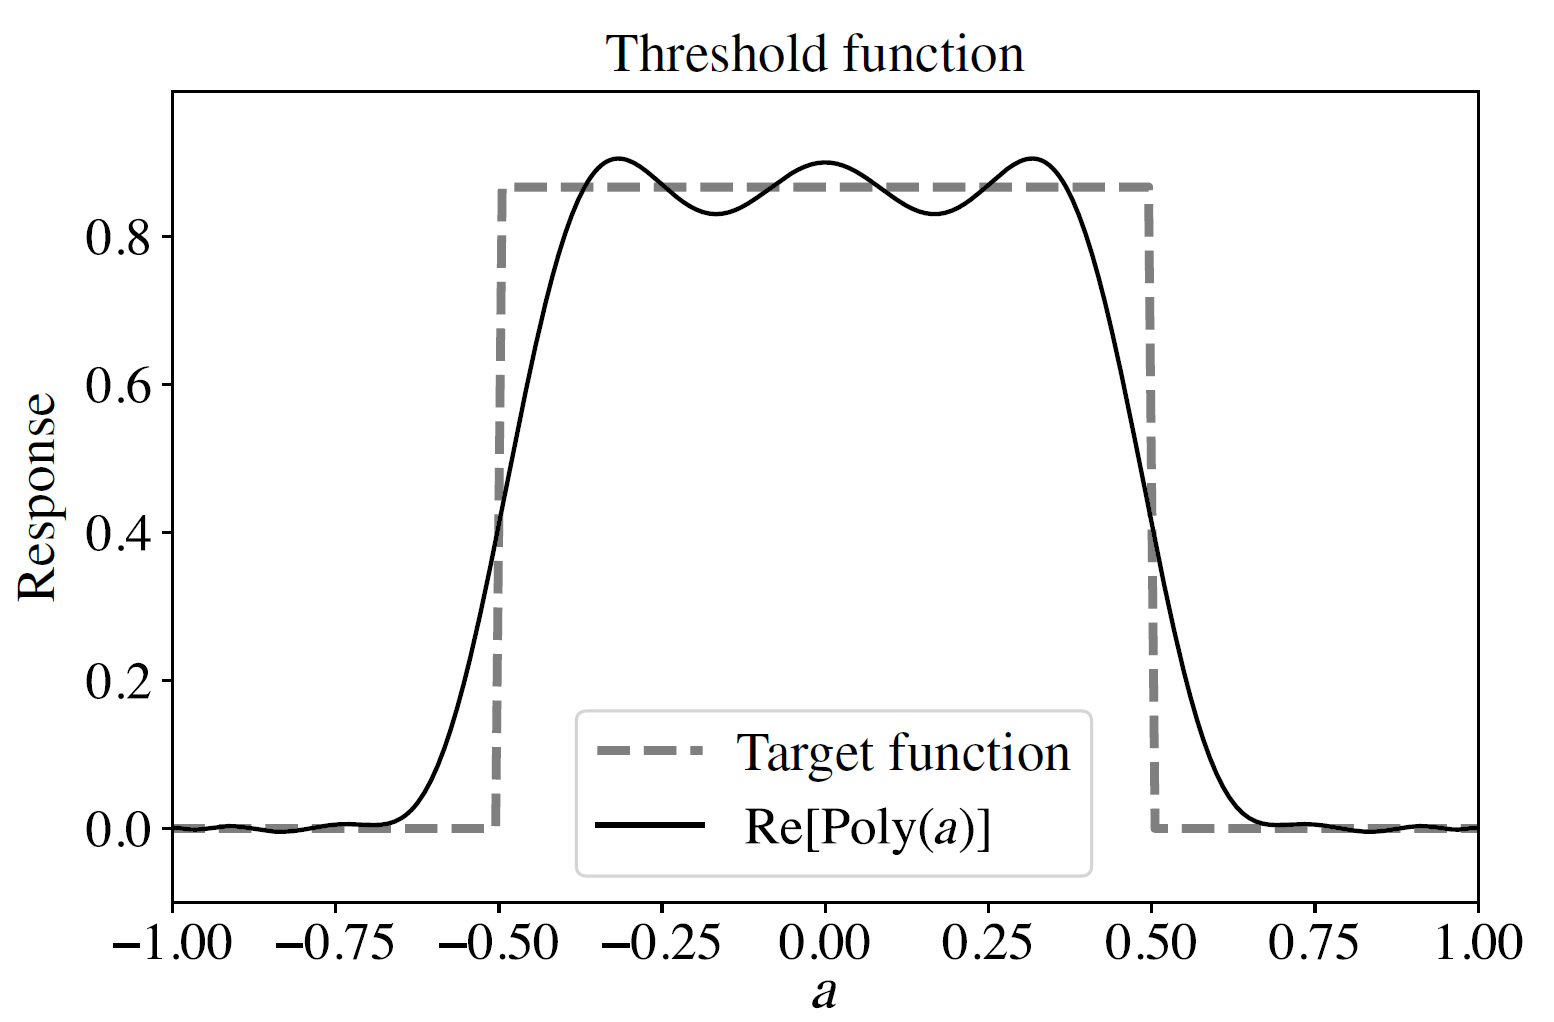
\includegraphics[width=0.4\textwidth]{qsp_threshold_poly_approx.png} & 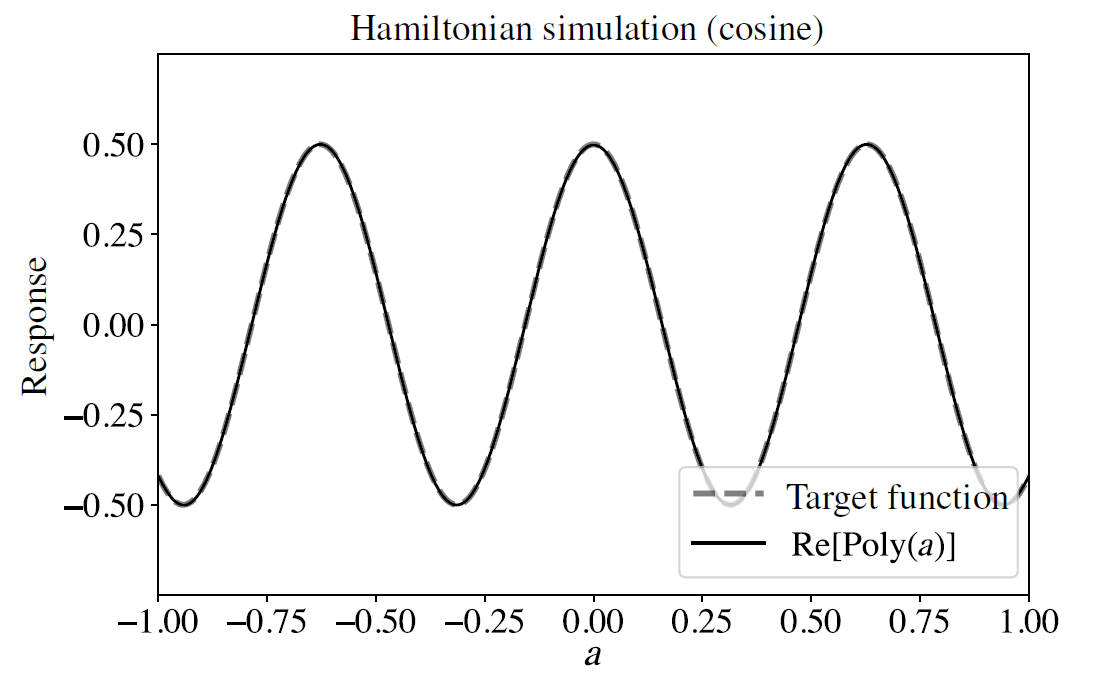
\includegraphics[width=0.4\textwidth]{qsp_hamiltonian_simulation.png} \\
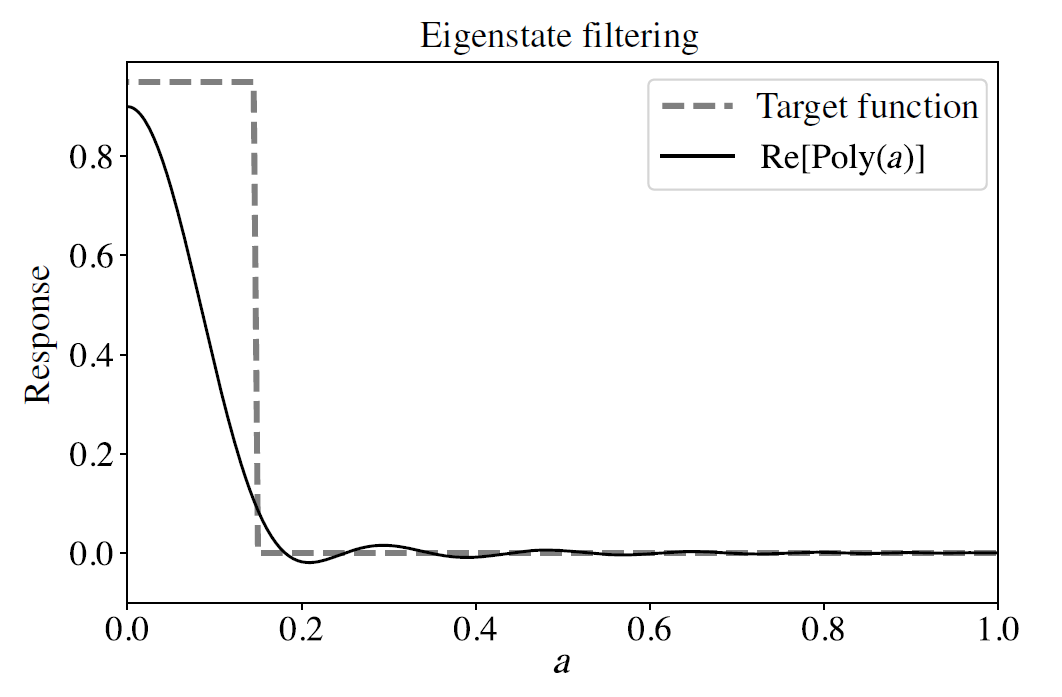
\includegraphics[width=0.4\textwidth]{qsp_eigenstate_filtering.png} & 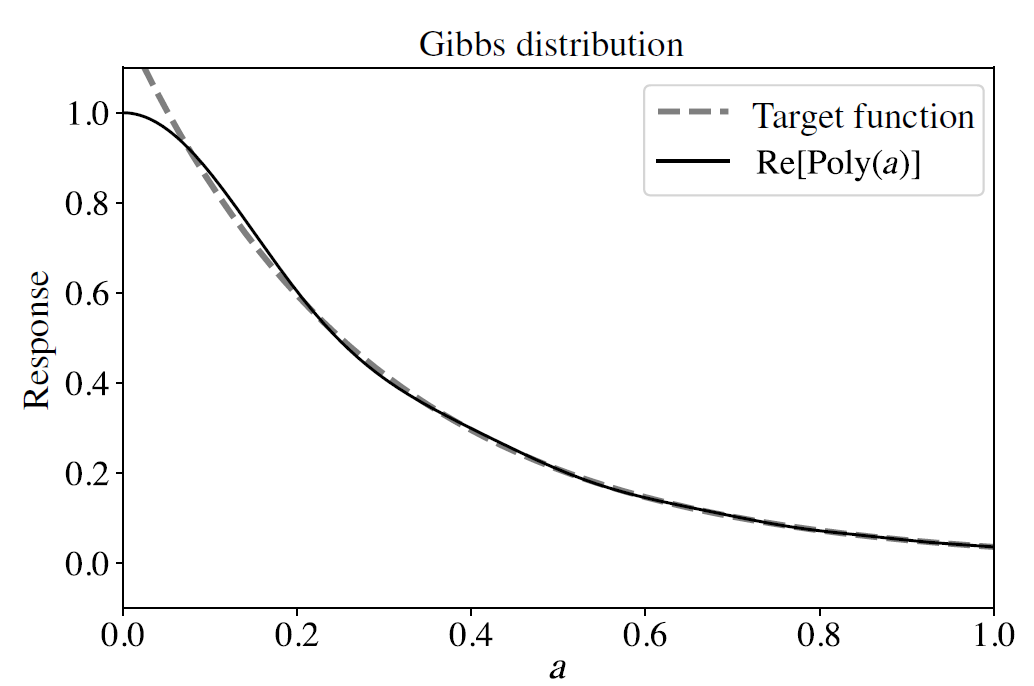
\includegraphics[width=0.4\textwidth]{qsp_gibbs.png}
\end{tabular}
\end{table}
\vspace{-1cm}
\footnotesize{%
{\usebeamercolor[fg]{structure}J.~M.~Martyn et al.} ``Grand unification of quantum algorithms''. PRX Quantum, 040203 (2021)\nocite{Martyn2021}%
}
\end{frame}



\PraesentationMasterWeissBlau

\begin{frame}
\vspace{7cm}
\begin{center}
{\LARGE Tensor network methods}

\vspace{1cm}

\begin{tikzpicture}[>=stealth, scale=1.5]
\foreach \x in {1,...,5}
{
    \node[draw, thick, inner sep=7, fill=TUMBlauHell, circle] (A\x) at (1.5*\x, 0) {};
    \coordinate (i\x) at (1.5*\x, -0.85);
    \draw[thick] (i\x) -- (A\x);
}
\foreach \x in {1,...,4}
{
    \pgfmathtruncatemacro{\z}{\x + 1};
    \draw[thick] (A\x) -- (A\z);
}
\end{tikzpicture}
\end{center}
\end{frame}

\PraesentationMasterStandard



\begin{frame}
\frametitle{Linear algebra: singular value decomposition}

\vspace{2cm}

\begin{theorem}[Singular value decomposition (SVD)]
Let $A \in \C^{n \times n}$ be a square matrix. Then there exist unitary matrices $U, V \in \C^{n \times n}$ and real numbers $\sigma_1, \dots, \sigma_n$ with $\sigma_1 \ge \cdots \ge \sigma_n \ge 0$ called \textbf{singular values}, such that
\[
A = U \begin{pmatrix} \sigma_1 & & \\ & \ddots & \\ & & \sigma_n \end{pmatrix} V^{\dagger}.
\]
\end{theorem}

Can be used to ``compress'' a matrix by discarding small singular values ($k \le n$):
\[
A \approx U \begin{pmatrix} \sigma_1 & & & & & \\ & \ddots & & & & \\ & & \sigma_k & & & \\ & & & 0 & & \\ & & & & \ddots & \\ & & & & & 0 \end{pmatrix} V^{\dagger} %
= U_{:, :k} \begin{pmatrix} \sigma_1 & & \\ & \ddots & \\ & & \sigma_k \end{pmatrix} V_{:, :k}^{\dagger}.
\]

{\small Demo: {\usebeamercolor[fg]{structure}\href{https://github.com/cmendl/edgar-luescher-seminar-2023/blob/master/notebooks/svd_compression.ipynb}{github.com/cmendl/edgar-luescher-seminar-2023/blob/master/notebooks/svd\_compression.ipynb}}}
\end{frame}



\begin{frame}
\frametitle{Tensors and graphical tensor diagrams}
\vspace{8cm}

Example: matrix-matrix multiplication

\vspace{4.5cm}

\footnotesize{%
{\usebeamercolor[fg]{structure}J.~C.~Bridgeman and C.~T.~Chubb} ``Hand-waving and interpretive dance: An introductory course on tensor networks''. J.~Phys.~A: Math.~Theor.~50, 223001 (2017)\nocite{BridgemanChubb2017}%
}
\end{frame}



\begin{frame}
\frametitle{Example: counting graph colorings}
\emph{Given a 3-regular graph, how many edge colorings using three colors exist, such that the edges at each vertex have distinct colors?}

\begin{center}
\begin{tikzpicture}[scale=1.75]
    \node[shape=circle, draw=black] (A) at ( 0, 0) {};
    \node[shape=circle, draw=black] (B) at ( 0, 1) {};
    \path[thick] (A) edge                (B);
    \path[thick] (A) edge[bend left=60]  (B);
    \path[thick] (A) edge[bend right=60] (B);
\end{tikzpicture}
\hspace{1cm}
\raisebox{9mm}{$\leadsto$}
\hspace{1cm}
\begin{tikzpicture}[scale=1.75]
    \node[shape=circle, draw=black] (A) at ( 0, 0) {};
    \node[shape=circle, draw=black] (B) at ( 0, 1) {};
    \path[thick, TUMBlau]   (A) edge                (B);
    \path[thick, TUMOrange] (A) edge[bend left=60]  (B);
    \path[thick, TUMGruen]  (A) edge[bend right=60] (B);
\end{tikzpicture}
\hspace{1cm}
\begin{tikzpicture}[scale=1.75]
    \node[shape=circle, draw=black] (A) at ( 0, 0) {};
    \node[shape=circle, draw=black] (B) at ( 0, 1) {};
    \path[thick, TUMBlau]   (A) edge                (B);
    \path[thick, TUMGruen]  (A) edge[bend left=60]  (B);
    \path[thick, TUMOrange] (A) edge[bend right=60] (B);
\end{tikzpicture}
\hspace{1cm}
\begin{tikzpicture}[scale=1.75]
    \node[shape=circle, draw=black] (A) at ( 0, 0) {};
    \node[shape=circle, draw=black] (B) at ( 0, 1) {};
    \path[thick, TUMOrange] (A) edge                (B);
    \path[thick, TUMBlau]   (A) edge[bend left=60]  (B);
    \path[thick, TUMGruen]  (A) edge[bend right=60] (B);
\end{tikzpicture}
\hspace{1cm}
\begin{tikzpicture}[scale=1.75]
    \node[shape=circle, draw=black] (A) at ( 0, 0) {};
    \node[shape=circle, draw=black] (B) at ( 0, 1) {};
    \path[thick, TUMOrange] (A) edge                (B);
    \path[thick, TUMGruen]  (A) edge[bend left=60]  (B);
    \path[thick, TUMBlau]   (A) edge[bend right=60] (B);
\end{tikzpicture}
\hspace{1cm}
\begin{tikzpicture}[scale=1.75]
    \node[shape=circle, draw=black] (A) at ( 0, 0) {};
    \node[shape=circle, draw=black] (B) at ( 0, 1) {};
    \path[thick, TUMGruen]  (A) edge                (B);
    \path[thick, TUMBlau]   (A) edge[bend left=60]  (B);
    \path[thick, TUMOrange] (A) edge[bend right=60] (B);
\end{tikzpicture}
\hspace{1cm}
\begin{tikzpicture}[scale=1.75]
    \node[shape=circle, draw=black] (A) at ( 0, 0) {};
    \node[shape=circle, draw=black] (B) at ( 0, 1) {};
    \path[thick, TUMGruen]  (A) edge                (B);
    \path[thick, TUMOrange] (A) edge[bend left=60]  (B);
    \path[thick, TUMBlau]   (A) edge[bend right=60] (B);
\end{tikzpicture}
\end{center}

Interpreted as tensor network, how to define tensors such that contracting the network gives the number of edge colorings?

\begin{tikzpicture}[scale=1.75]
    \node[shape=circle, draw=black] (T) at ( 0, 0) {\small $t$};
    \path[thick] (T) edge ( 0, 0.75);
    \path[thick] (T) edge ({0.75*cos(-30)}, {0.75*sin(-30)});
    \path[thick] (T) edge ({0.75*cos(210)}, {0.75*sin(210)});
\end{tikzpicture}

\begin{center}
\begin{tikzpicture}[scale=1.75]
    \node[shape=circle, draw=black] (A) at ( 0.866025, -0.5) {};
    \node[shape=circle, draw=black] (B) at ( 0.866025,  0.5) {};
    \node[shape=circle, draw=black] (C) at ( 0,         1  ) {};
    \node[shape=circle, draw=black] (D) at (-0.866025,  0.5) {};
    \node[shape=circle, draw=black] (E) at (-0.866025, -0.5) {};
    \node[shape=circle, draw=black] (F) at ( 0,        -1  ) {};
    \path (A) edge (B);
    \path (B) edge (C);
    \path (C) edge (D);
    \path (D) edge (E);
    \path (E) edge (F);
    \path (F) edge (A);
    \path (A) edge (D);
    \path (B) edge (E);
    \path (C) edge (F);
\end{tikzpicture}
\end{center}
\end{frame}



\begin{frame}
\frametitle{Matrix product states (MPS)}
\begin{tikzpicture}[>=stealth]
\node at (-5,0) {Lattice (1D):};
\foreach \x in {1,...,5}
{
    \fill (1.5*\x,0) circle (0.1);
    \node at (1.5*\x, -0.4) {{\small\x}};
}
\coordinate (S1) at (1.55,0.1);
\node (L) at (5, 0.6) {\small 2 spins (one qubit) per site};
\draw[thick, ->] (L) to [out=180,in=70] (S1);
\end{tikzpicture}
\begin{flalign*}
&\text{Wavefunction:} \qquad \Psi = \sum_{i \in \{0,1\}^{{\color{TUMBlau}N}}} \Psi_{i_1, \dots, i_{\color{TUMBlau}N}} \ket{i_1, \dots, i_{\color{TUMBlau}N}} &&
\end{flalign*}
\begin{minipage}[t]{0.55\textwidth}
Exact representation:
\end{minipage}%
\begin{minipage}[t]{0.4\textwidth}
MPS approximation:
\end{minipage}
\vspace{-0.5cm}
\begin{center}
\begin{tikzpicture}[>=stealth, scale=1.5]
\foreach \x in {1,...,5}
{
    \node[draw, thick, inner sep=1.5, fill=TUMBlauHell, circle] (A\x) at (1.5*\x, 0) {$A^\x$};
    \node (i\x) at (1.5*\x, -1) {$i_\x$};
    \draw[thick] (i\x) -- (A\x);
    \pgfmathtruncatemacro{\s}{\x - 6.5};
    \node (j\x) at (1.5*\s, -1) {$i_\x$};
    \draw[thick] (j\x) -- (1.5*\s, 0);
}
\foreach \x in {1,...,4}
{
    \pgfmathtruncatemacro{\z}{\x + 1};
    \draw[thick] (A\x) -- (A\z);
}
\draw[thick, fill=TUMBlauHell, rounded corners] (-7.75, -0.25) rectangle (-1.25, 0.25);
\node at (-4.5, 0) {$\Psi$};
\node (VL) at (4, 1) {\color{TUMGrau}virtual bond dim $D$};
\draw[->, thick, TUMGrau] (VL) to [out=190,in=90] (2.25, 0);
\draw[->, thick, TUMGrau] (VL) to [out=250,in=90] (3.75, 0);
\draw[->, thick, TUMGrau] (VL) to [out=340,in=90] (5.25, 0);
\draw[->, thick, TUMGrau] (VL) to [out=0,  in=90] (6.75, 0);
\end{tikzpicture}
\end{center}
\[
\hspace{1.5cm} \Psi_{i_1, \dots, i_{\color{TUMBlau}N}} \approx A^{(1)}_{i_1} \cdot A^{(2)}_{i_2} \cdots A^{({\color{TUMBlau}N})}_{i_{\color{TUMBlau}N}}
\]
\begin{minipage}[t]{0.55\textwidth}
{\color{TUMOrange}$\exp(N)$ many numbers}
\end{minipage}%
\begin{minipage}[t]{0.4\textwidth}
{\color{forestgreen}$\text{poly}(D, N)$ numbers}

\medskip

Why a good approximation?

$D$ bounded for typical $\Psi$
\end{minipage}
\end{frame}



\begin{frame}
\frametitle{Area law of the entanglement entropy}

\begin{figure}
\begin{tikzpicture}[>=stealth]
\foreach \x in {0,...,3}
{
    \fill (\x,0) circle (0.1);
}
\foreach \x in {-3,...,-1}
{
    \fill[gray] (\x,0) circle (0.1);
}
\foreach \x in {4,...,6}
{
    \fill[gray] (\x,0) circle (0.1);
}
\draw[dashed, ultra thick, forestgreen] (-0.5, -0.5) -- (-0.5, 0.5);
\draw[dashed, ultra thick, forestgreen] ( 3.5, -0.5) -- ( 3.5, 0.5);
\draw[very thick, <->] (0, -0.5) -- (3, -0.5);
\node at (1.5, -0.8) {$L$};
\node at (1.5,  0.5) {$A$};
\node at (5,  0.5) {${\color{gray}E}$};
\node at (-2, 0.5) {${\color{gray}E}$};
\end{tikzpicture}%
\hspace{0.1\textwidth}%
\begin{tikzpicture}[>=stealth]
\foreach \x in {0,...,6}
{
    \foreach \y in {1,...,5}
    {
        \fill[gray] (\x, \y) circle (0.1);
    }
}
\foreach \x in {2,...,4}
{
    \foreach \y in {2,...,4}
    {
        \fill (\x, \y) circle (0.1);
    }
}
\draw[dashed, ultra thick, forestgreen] (1.5, 1.5) rectangle (4.5, 4.5);
\draw[very thick, <->] (1.75, 1.75) -- (4.25, 1.75);
\node at (3.5, 1.4) {$L$};
\node at (3.5, 3.5) {$A$};
\node at (5.5, 4.5) {${\color{gray}E}$};
\end{tikzpicture}
\end{figure}
{\color{TUMBlau}Entanglement entropy:}
\[
S(L) = -\tr[\rho_A \log(\rho_A)] \quad \text{with} \quad \rho_A = \tr_E[\lvert\psi\rangle \langle\psi\rvert]
\]

Required bond dimension: $D \sim \e^{S(L)}$

\begin{table}
\begin{tabular}{p{0.45\textwidth} p{0.15\textwidth} l}
General random $\lvert\psi\rangle$ on a $d$-dim lattice & ${\color{TUMOrange}S(L) \sim L^d}$ & (volume) \\[0.5em]
Critical ground state on a 1D lattice & $S(L) \sim \log(L)$ & \\[0.5em]
Ground state for local $H$ on a $d$-dim lattice & ${\color{forestgreen}S(L) \sim L^{d-1}}$ & ({\color{forestgreen}area law})
\end{tabular}
\end{table}

Thus ${\color{forestgreen}S(L) = \text{const}}$, ${\color{forestgreen}D = \text{const}}$ for local $H$ on a 1D lattice!
\end{frame}


\begin{frame}
\frametitle{DMRG algorithm}
\vspace{1cm}

\begin{center}
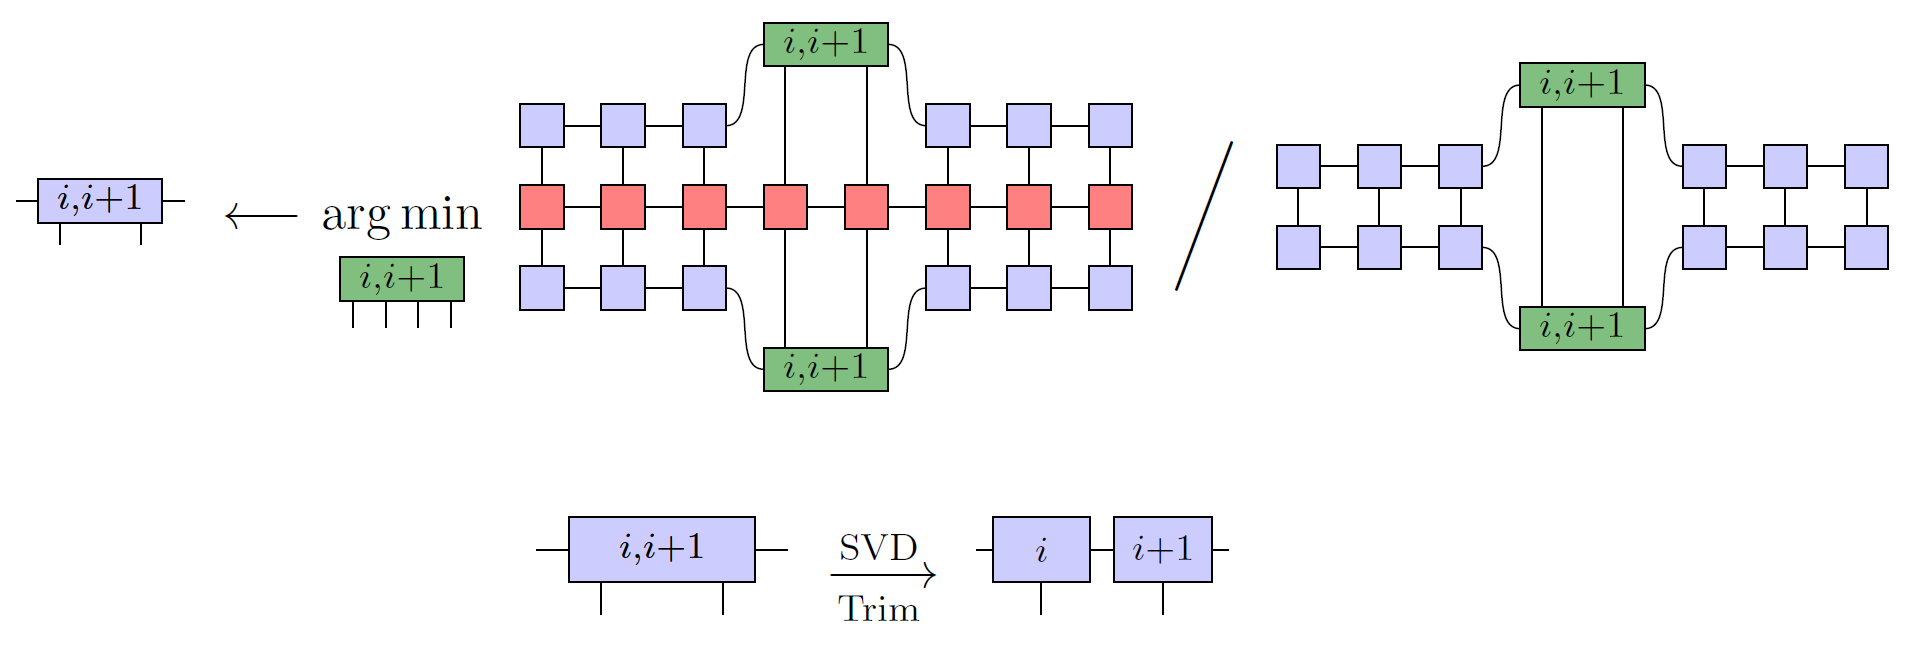
\includegraphics[width=\textwidth]{dmrg_step.png}\\
{\small Image source: Bridgeman and Chubb (2017)}
\end{center}

{\small Demo: {\usebeamercolor[fg]{structure}\href{https://github.com/cmendl/edgar-luescher-seminar-2023/blob/master/notebooks/mps_ground_state.ipynb}{github.com/cmendl/edgar-luescher-seminar-2023/blob/master/notebooks/mps\_ground\_state.ipynb}}}

{\footnotesize
{\usebeamercolor[fg]{structure}J.~C.~Bridgeman and C.~T.~Chubb} ``Hand-waving and interpretive dance: An introductory course on tensor networks''. J.~Phys.~A: Math.~Theor.~50, 223001 (2017)\nocite{BridgemanChubb2017}\\
{\usebeamercolor[fg]{structure}U.~Schollw\"ock} ``The density-matrix renormalization group in the age of matrix product states''. Ann.~Physics 326, 96--192 (2011)\nocite{Schollwoeck2011}%
}
\end{frame}



\begin{frame}
\frametitle{References}
{\small
\printbibliography
}
\end{frame}



\end{document}
